\documentclass{article}
\usepackage[utf8]{inputenc}
\usepackage[left=2cm,right=10cm,top=2cm,bottom=2cm]{geometry}

\usepackage[T2A]{fontenc}
\usepackage[utf8]{inputenc}
\usepackage[russian]{babel}
\usepackage{amssymb}
\usepackage{multicol}
\usepackage{amsmath}
\usepackage{tikz}
\usepackage{graphicx}
\graphicspath{ {./} }

\usepackage[shortlabels]{enumitem}

\begin{document}


Пусть $X= (A \setminus B) \cap C$  – некоторое множество. Выберите равные ему множества.

$$ Y = B \setminus (A \cap (C \cup (A \cap B)))$$

$$Y = C \bigtriangleup ((\overline{B} \cup C) \cap (\overline{A} \cup \overline{B}))$$

$$Y = (((C \cup B) \cup A) \setminus B) \cup \overline{A}$$

$$Y = ((C \bigtriangleup B) \cap C) \cap \overline{(\overline{B} \setminus A)}$$


$$Y = (C \cup B) \cap (A \bigtriangleup (B \cap A))$$


\textbf{Решение}

На кругах Эйлера

$$X= (A \setminus B) \cap C$$

\begin{enumerate}
    \item $(A \setminus B)$
    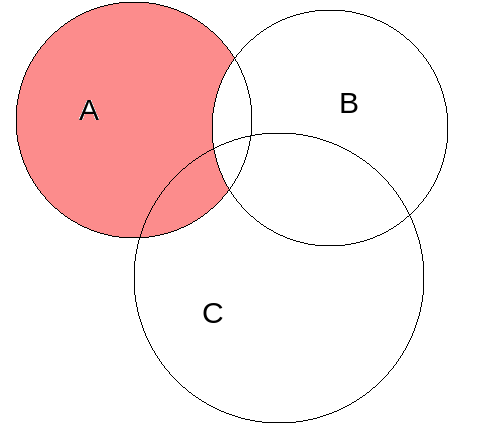
\includegraphics[width=50mm]{1.png}
    
    \item $(A \setminus B) \cap C$
    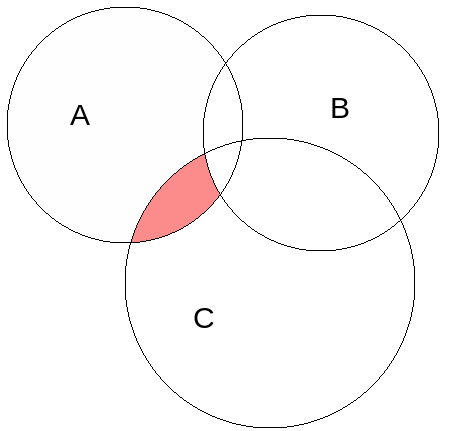
\includegraphics[width=50mm]{2.png}
\end{enumerate}

\noindent\makebox[\linewidth]{\rule{\paperwidth}{0.4pt}}

$$ Y = B \setminus (A \cap (C \cup (A \cap B)))$$

\begin{enumerate}
    \item $(A \cap B)$
    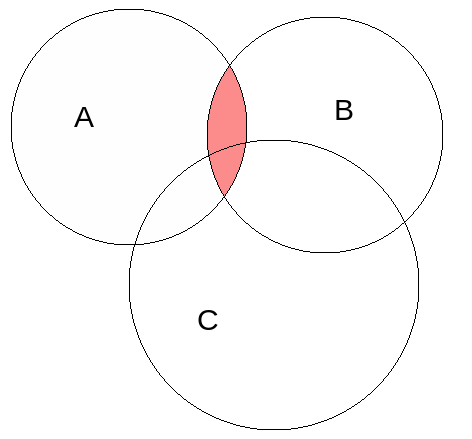
\includegraphics[width=50mm]{3.png}
    
    \item $(C \cup (A \cap B))$
    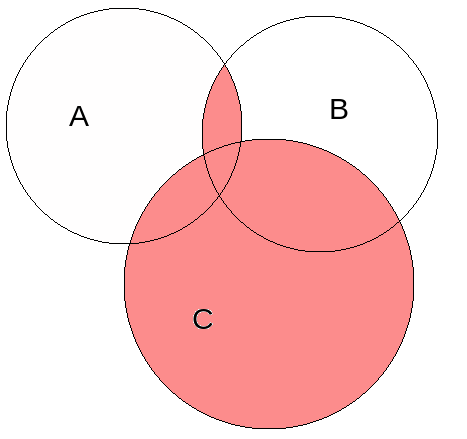
\includegraphics[width=50mm]{4.png}
    
    \item $(A \cap (C \cup (A \cap B)))$
    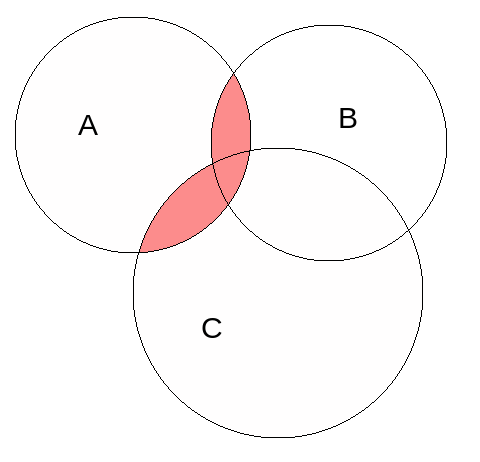
\includegraphics[width=50mm]{5.png}
    
    \item $B \setminus (A \cap (C \cup (A \cap B)))$
    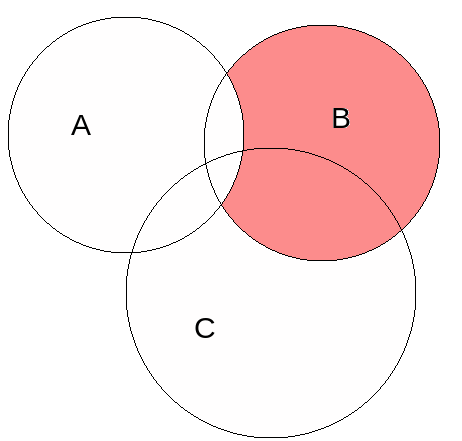
\includegraphics[width=50mm]{6.png}
\end{enumerate}

\noindent\makebox[\linewidth]{\rule{\paperwidth}{0.4pt}}

$$Y = C \bigtriangleup ((\overline{B} \cup C) \cap (\overline{A} \cup \overline{B}))$$

\begin{enumerate}
    \item $\overline{A}$
    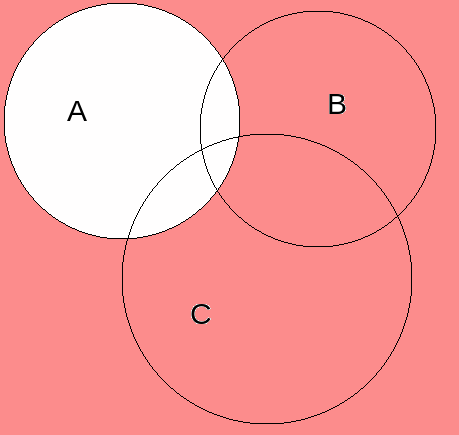
\includegraphics[width=50mm]{7.png}
    
    \item $\overline{B}$
    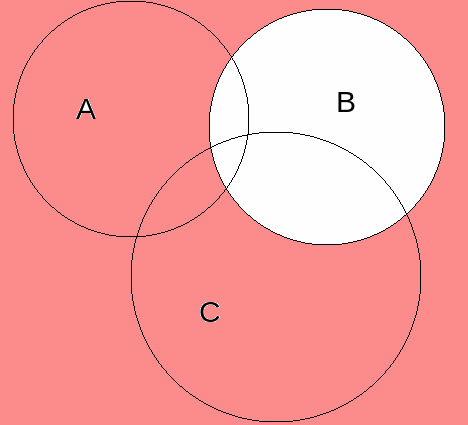
\includegraphics[width=50mm]{8.png}
    
    \item $(\overline{A} \cup \overline{B})$
    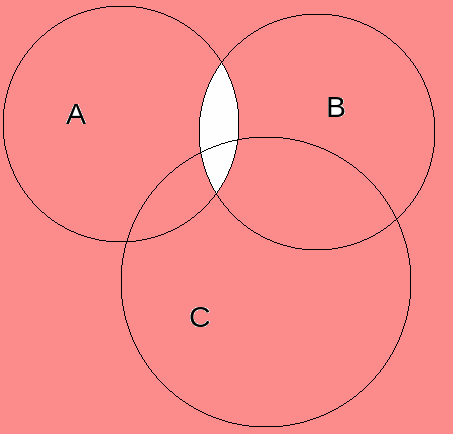
\includegraphics[width=50mm]{9.png}
    
    \item $(\overline{B} \cup C)$
    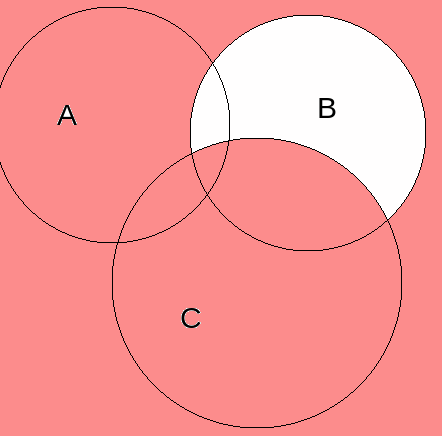
\includegraphics[width=50mm]{10.png}

    \item $((\overline{B} \cup C) \cap (\overline{A} \cup \overline{B}))$
    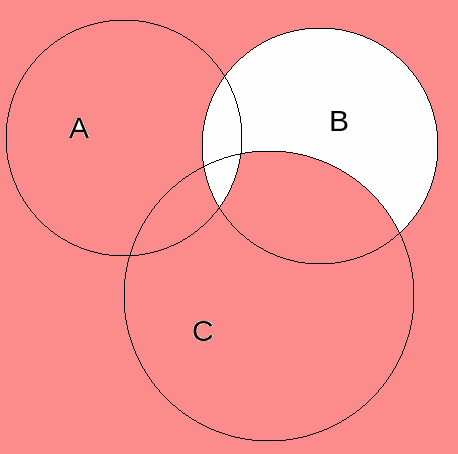
\includegraphics[width=50mm]{11.png}
    
    \item $C \bigtriangleup ((\overline{B} \cup C) \cap (\overline{A} \cup \overline{B}))$
    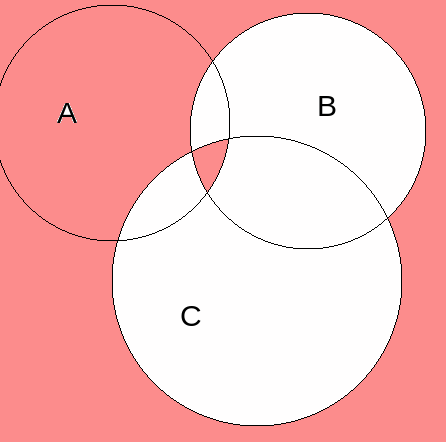
\includegraphics[width=50mm]{12.png}
\end{enumerate}

\noindent\makebox[\linewidth]{\rule{\paperwidth}{0.4pt}}


$$Y = (((C \cup B) \cup A) \setminus B) \cup \overline{A}$$

\begin{enumerate}
    \item $((C \cup B) \cup A)$
    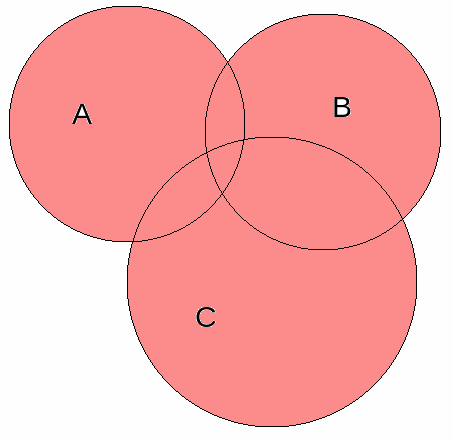
\includegraphics[width=50mm]{13.png}
    
    \item $((C \cup B) \cup A) \setminus B)$
    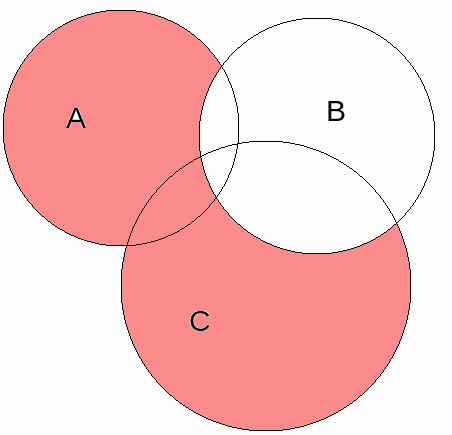
\includegraphics[width=50mm]{14.png}
    
    \item $(((C \cup B) \cup A) \setminus B) \cup \overline{A}$
    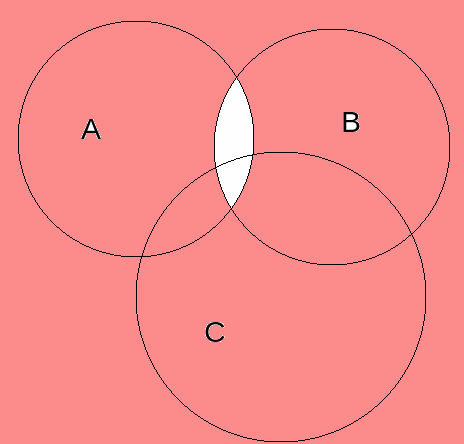
\includegraphics[width=50mm]{15.png}
\end{enumerate}


\noindent\makebox[\linewidth]{\rule{\paperwidth}{0.4pt}}
$$Y = ((C \bigtriangleup B) \cap C) \cap \overline{(\overline{B} \setminus A)}$$

\begin{enumerate}
    \item $(C \bigtriangleup B)$
    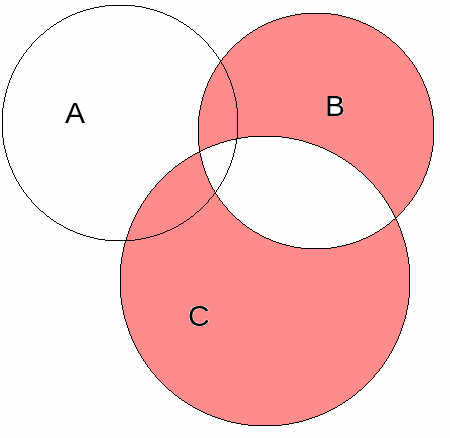
\includegraphics[width=50mm]{16.png}
    
    \item $((C \bigtriangleup B) \cap C)$
    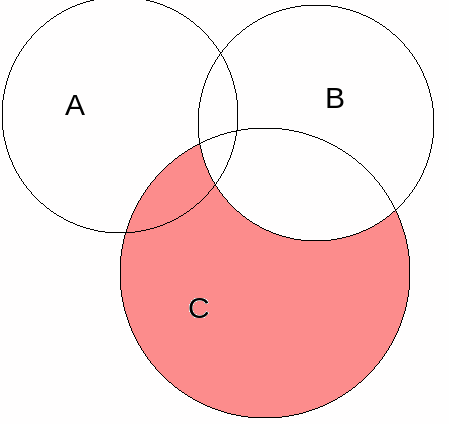
\includegraphics[width=50mm]{17.png}
    
    \item $(\overline{B} \setminus A)$
    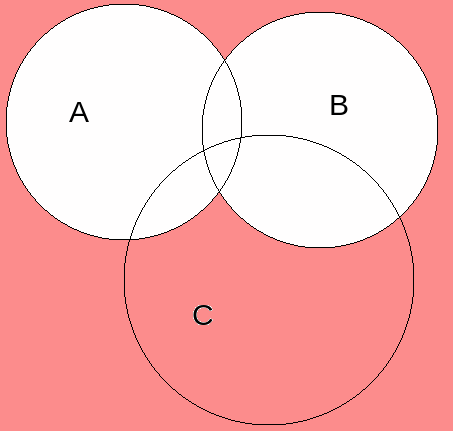
\includegraphics[width=50mm]{18.png}
    
    \item $\overline{(\overline{B} \setminus A)}$
    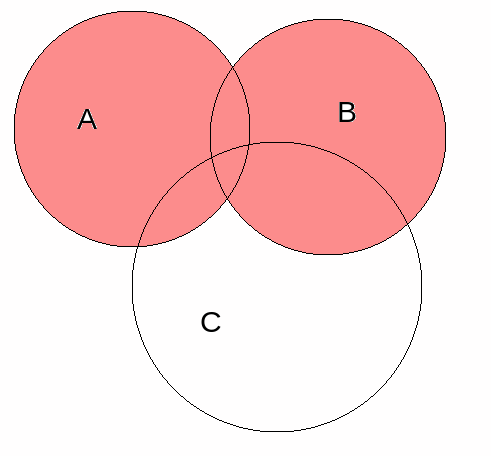
\includegraphics[width=50mm]{19.png}
    
    \item $((C \bigtriangleup B) \cap C) \cap \overline{(\overline{B} \setminus A)}$
    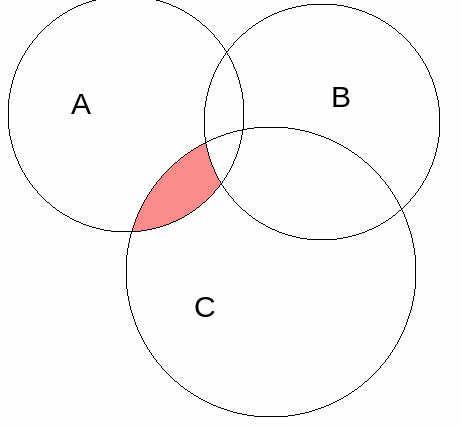
\includegraphics[width=50mm]{20.png}
\end{enumerate}


\noindent\makebox[\linewidth]{\rule{\paperwidth}{0.4pt}}
$$Y = (C \cup B) \cap (A \bigtriangleup (B \cap A))$$

\begin{enumerate}
    \item $(C \cup B)$
    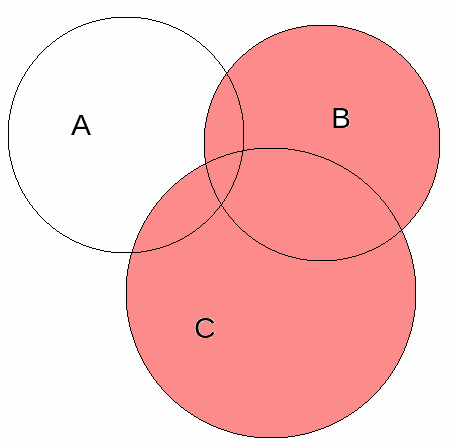
\includegraphics[width=50mm]{21.png}
    
    \item $(B \cap A)$
    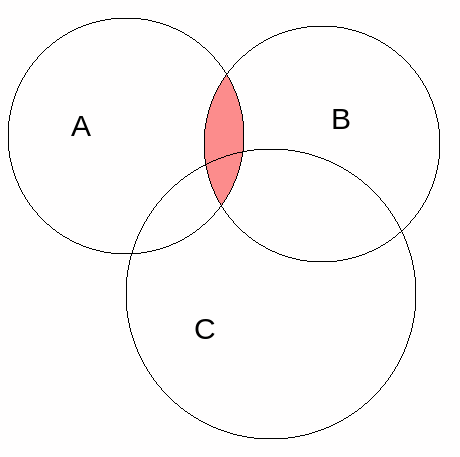
\includegraphics[width=50mm]{22.png}
    
    \item $(A \bigtriangleup (B \cap A))$
    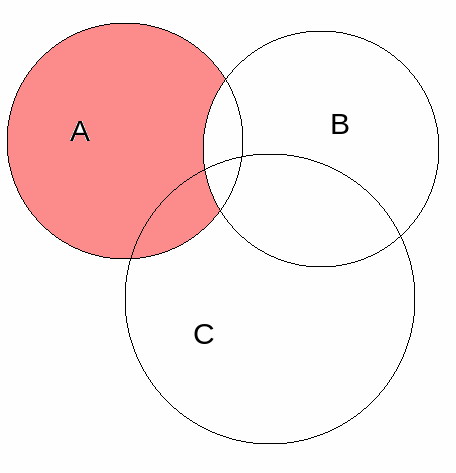
\includegraphics[width=50mm]{23.png}
    
    \item $(C \cup B) \cap (A \bigtriangleup (B \cap A))$
    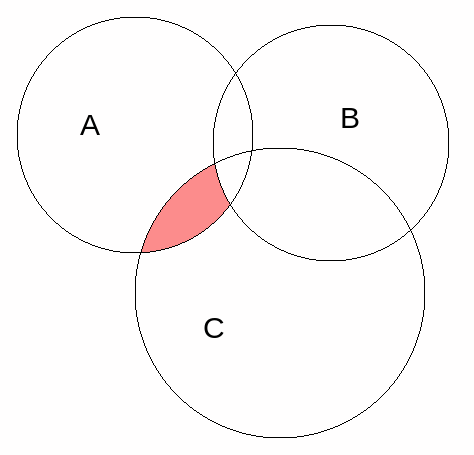
\includegraphics[width=50mm]{24.png}
\end{enumerate}


\end{document}
